\RequirePackage[l2tabu, orthodox]{nag}
% the nag package warns you for incorrect latex usage

\documentclass[a4j, titlepage, 10pt]{jsarticle}
% %% ----- page -----
\usepackage[utf8]{inputenc} % encoding
\usepackage{setspace} \setstretch{1.1} % set space between the lines
\usepackage[top=30truemm, bottom=30truemm, left=25truemm, right=25truemm]{geomet
ry} % page margins
% %% ----- math -----
% \usepackage{amsmath, amssymb}
% \renewcommand{\~}{$\sim$}
% %% ----- figure -----
% \usepackage{here}
\usepackage[dvipdfmx, hiresbb]{graphicx}
% %% ----- table -----
\usepackage{booktabs}
% \newcommand{\question}{?}
% \catcode63=\active \def?{\phantom{0}} % ? -> ' '
% %% ----- programing -----
% \usepackage{verbatim}
\newcommand{\code}[1]{\texttt{#1}}
% %% --- border ---
% \usepackage{fancybox, ascmac}
% %% --- listing ---
\usepackage{ascmac}
\usepackage{here}
\usepackage{txfonts}
\usepackage{listings} %, jlisting}
\renewcommand{\lstlistingname}{リスト}
\lstset{
  language = c,
  numbers = left,
  stepnumber = 1,
  numberstyle = \scriptsize,
  numbersep = 10pt,
  breaklines = true,
  breakindent = 20pt,
  lineskip = -0.2zw,
  frame = tRBl,
  framesep = 5pt,
  basicstyle = \ttfamily\small,
  commentstyle = \textit,
  keywordstyle = \bfseries,
  classoffset = 1,
  showstringspaces = false,
  tabsize = 2
}
% %% ----- others -----
% \usepackage{url} % \url{url_path}

% 何を作ったか
% どういう風に動作するか
% 画面のキャプチャ
% 工夫した点
% 大変だったところ
% ソースコード(自分の作った部分だけでも良いがなるべく載せる)


\begin{document}
% begin title
\title{{ \Huge ネットワークプログラミングII }~\\{ \LARGE 総合演習 }}
\author{{ \Large 402 } \and { \Large 411 }}
\date{\today}
\maketitle
% end title

% ==============================================================================
\section{概要}

今回、ネットワークプログラミングIIの総合演習として作成した作品は「六目並べ」である。
% TODO: 六目並べの説明
初めに、六目並べについて説明する。これに似たゲームとして、五目並べが挙げられる。しかしながら、五目並べは先手必勝であることが証明されている。先手においては、6個以上の石の連である長連、同一衝点に四が2個以上同時にできるものである四四、同一衝点に三が2個以上同時にできるものである三三は反則負けとされているが、それでも先手必勝は変わらない。この不公平さを解消するために考案されたのが六目並べである。
% TODO: どういう風に動作するか

続いて、六目並べのゲームの流れを次に示す。
\begin{enumerate}
  \item 先手が1回打つ
  \item 後手が2回打つ
  \item 先手が2回打つ
  \item 2〜3を先手と後手のどちらかが6個の石の連を作るまで続ける
\end{enumerate}
このルールに則ることで、先手後手による不公平さが五目並べよりも少なくなる。

% ==============================================================================
\section{ソースコード}

総合演習で作成したソースコードをリスト\ref{code:sessionman.h}~\ref{code:client.c}に示す。
sessionman.hであるリスト\ref{code:sessionman.h}では、sessionman.cで使用するマクロや外部関数を宣言した。
なお、このプログラムを実行するにはサーバの50002番ポートを開けておく必要がある。

\lstset{ numbers = left }
\lstinputlisting[caption=sessionman.h,label=code:sessionman.h]{../sessionman.h}

sessionman.cであるリスト\ref{code:sessionman.c}では、セッションに関する処理の定義をした。
サーバーに接続した各クライアントには各ファイルディスクリプタfdが割り当てられ、サーバとクライアントはfdを通して通信を行う。
15行目から18行目では各クライアントの情報を格納する構造体ATTENDANTを定義した。
25行目のenter関数では、i番目のクライアントを割り当てられたfdで初期化する処理を行う。
38行目のsessionman\_init関数では、ゲームの先攻後攻を決める処理を行う。これはゲームが開始するときに呼び出される。
63行目のsessionman\_loop関数では、各クライアントから送られてきた内容を全てのクライアントに送信する処理を行う。
89行目のending関数では、サーバとクライアントの通信の終了処理を行う。
101行目のsend\_all関数では、全てのクライアントにグローバル変数bufの内容を送信する処理を行う。

\lstset{ numbers = left }
\lstinputlisting[caption=sessionman.c,label=code:sessionman.c]{../sessionman.c}

session.hであるリスト\ref{code:session.h}では、session.cで使用するマクロや外部関数を宣言した。

\lstset{ numbers = left }
\lstinputlisting[caption=session.h,label=code:session.h]{../session.h}

session.cであるリスト\ref{code:session.c}では、六目並べのゲームの処理とサーバと通信を行う処理を行う。
58行目のsession\_init関数ではソケットの初期化と、ゲームのために使用するライブラリncursesの初期化を行う。
93行目のsession\_loop関数では、プレイヤーやサーバからの入力を監視するためのループを行う。
109行目のif文以降では、標準入力から入力があった場合の処理を行う。
標準入力からのキーの入力に対応する処理を表\ref{tab:player-key-mapping}に示す。
148行目のif文以降では、サーバからデータが送られてきた場合の処理を行う。
具体的に、送られてきた文字列とそれに対応する処理を表\ref{tab:mapping-received-str-and-corresponding-process}に示す。

session.cであるリスト\ref{code:session.c}のプライベート関数について、
226行目のinit\_goban関数では、碁盤の初期化を行う。
243行目のis\_my\_turn関数では、ゲームのステップ数と自分の石の文字を与えると、
現在のターンが自分のターンであれば1を、相手のターンであれば0を返す。
256行目のput\_stone関数では、与えられた(x,y)座標に石が何も置かれていない場合に、
与えられた石の文字を碁盤に配置する。
267行目のdie関数では、ゲーム終了時の処理を行う。
274行目のdetect\_rokumoku関数では、与えられた石の文字列が碁盤上で6つ以上ならんでいるかを調べる。
石が6つ以上ならんでいれば1を、そうでなければ0を返す。

\lstset{ numbers = left }
\lstinputlisting[caption=session.c,label=code:session.c]{../session.c}

\begin{table}[H]
  \centering
  \caption{プレイヤーからのキーの入力に対応する処理}
  \label{tab:player-key-mapping}
  \begin{tabular}{ll} \toprule
    キーの入力 & 行う処理 \\
    \midrule
    j & 一つ下へカーソルを移動する \\
    k & 一つ上へカーソルを移動する \\
    h & 一つ左へカーソルを移動する \\
    l & 一つ右へカーソルを移動する \\
    space & 現在のカーソルの位置に石を置く \\
    r & ゲームをリセットする \\
    q & ゲームを終了する \\
    \bottomrule
  \end{tabular}
\end{table}

\begin{table}[H]
  \centering
  \caption{サーバから送られてきた文字列とそれに対応する処理}
  \label{tab:mapping-received-str-and-corresponding-process}
  \begin{tabular}{ll} \toprule
    送られてきた文字列 & 行う処理 \\
    \midrule
    \code{:$N$} & 数字$N$が1なら先攻、0なら後攻でゲーム開始 \\
    \code{($X$,$Y$) $C$} & 座標($X$,$Y$)の位置に文字$C$の石を置く \\
    \code{reset} & ゲームをリセットする \\
    \code{quit} & ゲームを終了する \\
    \bottomrule
  \end{tabular}
\end{table}

server.cであるリスト\ref{code:server.c}では、
サーバ側のプログラムを立ち上げた時にクライアント側からの通信を待ち、
2台のクライアントが接続したらゲームを開始するなどの一連の作業を行う。

\lstset{ numbers = left }
\lstinputlisting[caption=server.c,label=code:server.c]{../server.c}

client.cであるリスト\ref{code:client.c}では、
クライアント側のプログラムを立ち上げた時にサーバとソケット通信をするための処理を行い、
ゲームでのレンダリングやユーザ入力の処理などの一連の作業を行う。

\lstset{ numbers = left }
\lstinputlisting[caption=client.c,label=code:client.c]{../client.c}

最後に、作成したプログラムをコンパイルするMakefileをリスト\ref{code:Makefile}に示す。
リスト\ref{code:Makefile}のMakefileを使ってmakeすると、binディレクトリの下にsとcという実行ファイルができる。
なお、sとcはそれぞれサーバ用とクライアント用の実行ファイルであることを表している。

\lstset{ numbers = left }
\lstinputlisting[caption=Makefile,label=code:Makefile]{../Makefile}


% ==============================================================================
\section{実行結果}

まずサーバ側でbin/sを実行してからクライアント側となる2つ画面を用意して,それぞれでbin/cを実行した結果を
図\ref{fig:game-start1.png}と\ref{fig:game-start2.png}に示す。

% TODO: 実行結果の説明

\begin{figure}[H]
  \begin{minipage}{0.5\hsize}
    \centering
    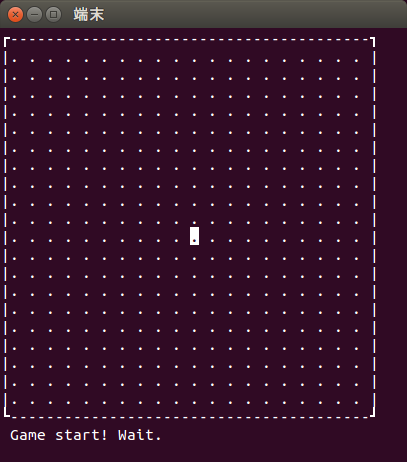
\includegraphics[scale=0.5]{img/game-start1.png}
    \caption{Caption}
    \label{fig:game-start1.png}
  \end{minipage}
  \begin{minipage}{0.5\hsize}
    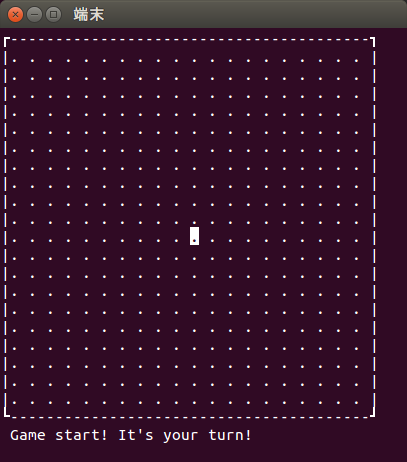
\includegraphics[scale=0.5]{img/game-start2.png}
    \caption{Caption}
    \label{fig:game-start2.png}
  \end{minipage}
\end{figure}
図\ref{fig:game-start1.png}は後手番となったときのゲーム開始直後の画面である。対して、図\ref{fig:game-start2.png}は先手番となったときのゲーム開始直後の画面である。{\ttfamily It's your turn!}と表示されたことから判別ができる。この盤面から先手が1回打ったときの画面を図\ref{fig:put1-1.png}と\ref{fig:put1-2.png}に示す。

\begin{figure}[H]
  \begin{minipage}{0.5\hsize}
    \centering
    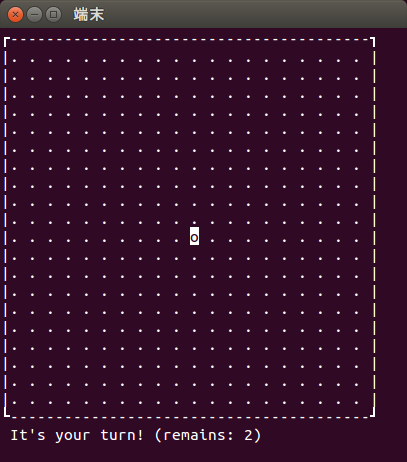
\includegraphics[scale=0.5]{img/put1-1.png}
    \caption{Caption}
    \label{fig:put1-1.png}
  \end{minipage}
  \begin{minipage}{0.5\hsize}
    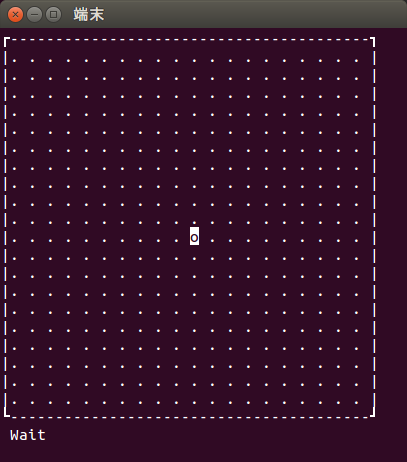
\includegraphics[scale=0.5]{img/put1-2.png}
    \caption{Caption}
    \label{fig:put1-2.png}
  \end{minipage}
\end{figure}
図\ref{fig:put1-1.png}より、自分の手番となったことが確認できる。先手が表\ref{tab:player-key-mapping}に則って打ったことで、盤面の{\ttfamily .}が{\ttfamily o}に変わっていることが確認できる。図\ref{fig:put1-2.png}で表される先手は、先ほど打ったために自分の手番ではない。この盤面から後手が1回打ったときの画面を図\ref{fig:put2-1.png}と\ref{fig:put2-2.png}に示す。

\begin{figure}[H]
  \begin{minipage}{0.5\hsize}
    \centering
    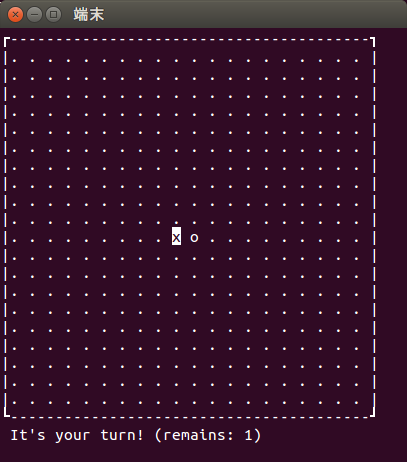
\includegraphics[scale=0.5]{img/put2-1.png}
    \caption{Caption}
    \label{fig:put2-1.png}
  \end{minipage}
  \begin{minipage}{0.5\hsize}
    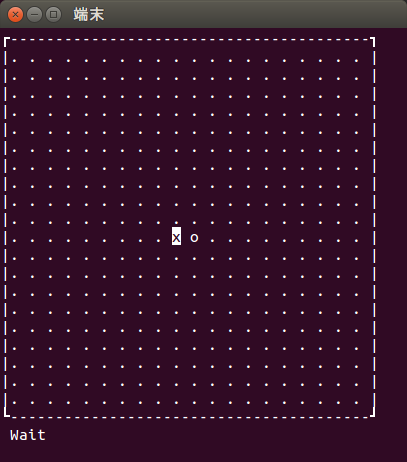
\includegraphics[scale=0.5]{img/put2-2.png}
    \caption{Caption}
    \label{fig:put2-2.png}
  \end{minipage}
\end{figure}
図\ref{fig:put2-1.png}より、盤面の{\ttfamily .}が{\ttfamily x}に変わり、打てる回数である{\ttfamily remains}が2から1に減っていることが確認できる。図\ref{fig:put2-2.png}で表される先手は、自分の手番ではない。この盤面から後手が1回打ったときの画面を図\ref{fig:put3-1.png}と\ref{fig:put3-2.png}に示す。

\begin{figure}[H]
  \begin{minipage}{0.5\hsize}
    \centering
    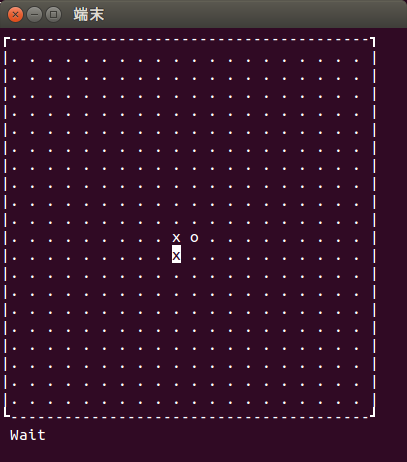
\includegraphics[scale=0.5]{img/put3-1.png}
    \caption{Caption}
    \label{fig:put3-1.png}
  \end{minipage}
  \begin{minipage}{0.5\hsize}
    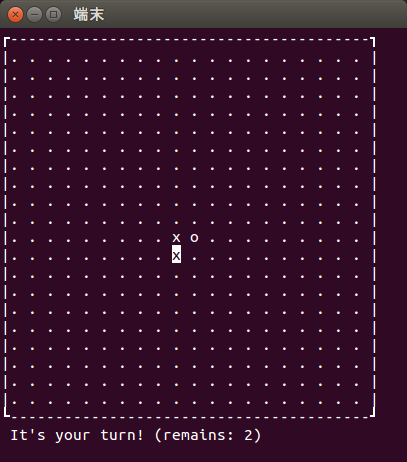
\includegraphics[scale=0.5]{img/put3-2.png}
    \caption{Caption}
    \label{fig:put3-2.png}
  \end{minipage}
\end{figure}
図\ref{fig:put3-1.png}より、盤面の{\ttfamily .}が{\ttfamily x}に変わり、打てる回数である{\ttfamily remains}が0になったために先手の手番となったことが確認できる。図\ref{fig:put3-2.png}で表される先手は、後手が2回打ったために自分の手番となった。この局面から交互に2回ずつ打っていったときの盤面を図\ref{fig:fin-prev1-1.png}と\ref{fig:fin-prev1-2.png}に示す。

\begin{figure}[H]
  \begin{minipage}{0.5\hsize}
    \centering
    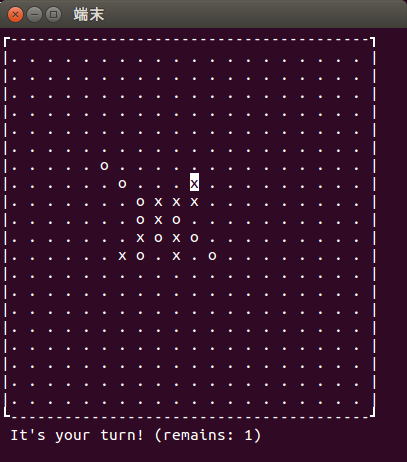
\includegraphics[scale=0.5]{img/fin-prev1-1.png}
    \caption{Caption}
    \label{fig:fin-prev1-1.png}
  \end{minipage}
  \begin{minipage}{0.5\hsize}
    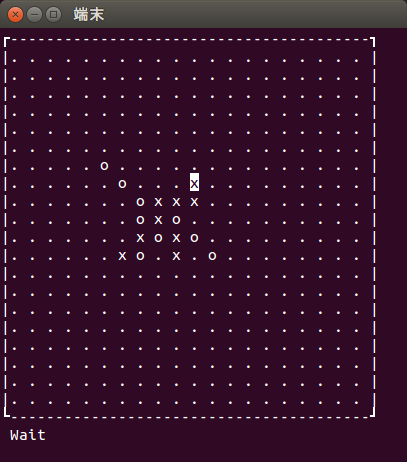
\includegraphics[scale=0.5]{img/fin-prev1-2.png}
    \caption{Caption}
    \label{fig:fin-prev1-2.png}
  \end{minipage}
\end{figure}

図\ref{fig:fin-prev1-1.png}と\ref{fig:fin-prev1-2.png}の状態から後手が6つ並べたときのようすを図\ref{fig:fin-1.png}、\ref{fig:fin-2.png}に示す。
\begin{figure}[H]
  \begin{minipage}{0.5\hsize}
    \centering
    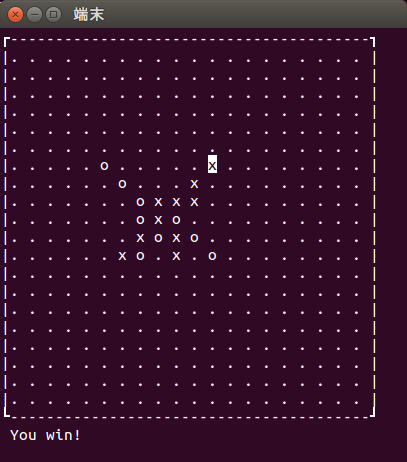
\includegraphics[scale=0.5]{img/fin-1.png}
    \caption{Caption}
    \label{fig:fin-1.png}
  \end{minipage}
  \begin{minipage}{0.5\hsize}
    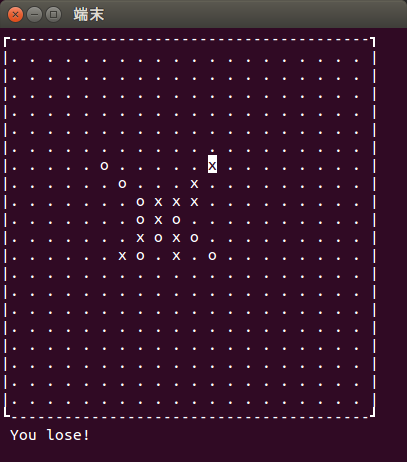
\includegraphics[scale=0.5]{img/fin-2.png}
    \caption{Caption}
    \label{fig:fin-2.png}
  \end{minipage}
\end{figure}
図\ref{fig:fin-1.png}より、カーソルのある地点から左斜め下に向かって6つ{\ttfamily x}が並んでおり、{\ttfamily You win!}と表示されていることが確認できる。対して、図\ref{fig:fin-2.png}より、{\ttfamily You lose!}と表示されていることが確認できる。以上が作成した六目並べの一連の流れである。

% ==============================================================================
\section{考察}

% TODO: 工夫した点
% TODO: 大変だったところ


\end{document}
